% with xelatex
\documentclass[border=1pt]{standalone}

%\usepackage[utf8]{inputenc}
%\usepackage[T1]{fontenc}

%\usepackage{upgreek}
%\usepackage{arev}
%\usepackage{helvet}
%\usepackage{graphicx}
\usepackage{tikz}
\usepackage{tkz-euclide}
%\usepackage{pst-solides3d}
%\usepackage{auto-pst-pdf}
\usetikzlibrary{calc,decorations.pathmorphing,shapes,backgrounds,arrows.meta,arrows,automata,positioning}

%\renewcommand{\familydefault}{\sfdefault}

\usepackage{mathspec}
%\setallmainfonts{Linux Libertine O}
\setallmainfonts{Arial}

\begin{document}

  \begin{tikzpicture}
    \node at (-5,0) {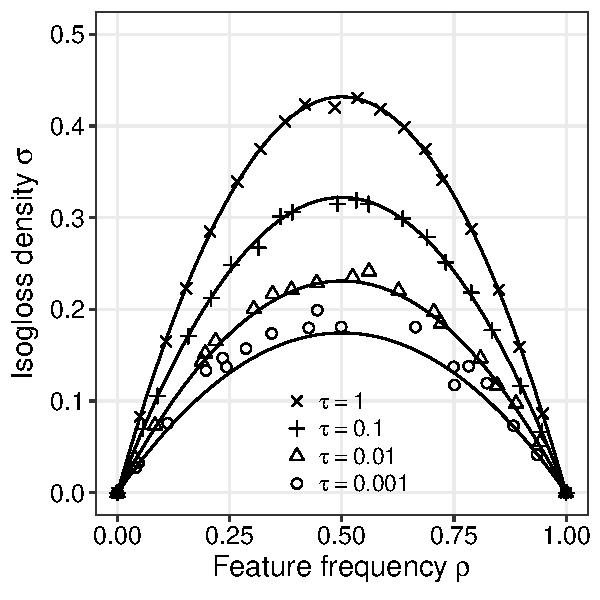
\includegraphics[scale=0.8]{newsimutheory}};
    \node at (4.2,0) {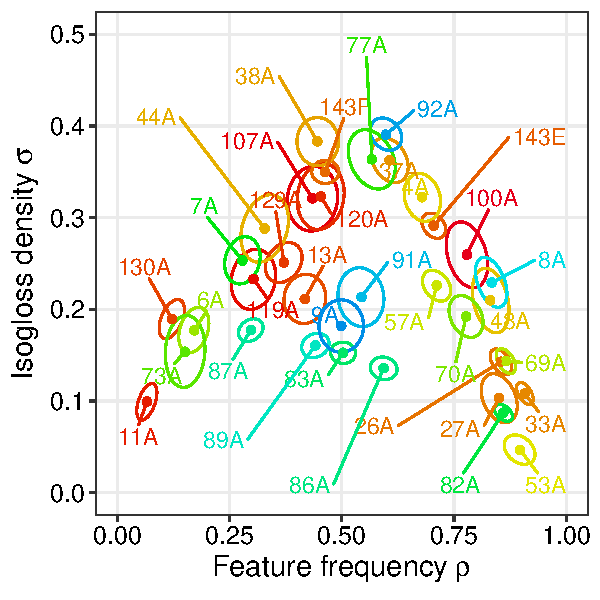
\includegraphics[scale=0.8]{newmain}};
    \setlength{\fboxsep}{0pt}
    \node at (-7.3,3.15) {\fbox{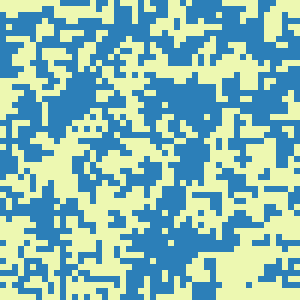
\includegraphics[width=2.2cm]{snapshot1}}};
    %\draw (-5.6,4.2) rectangle (-3.6,2.2);
    \draw (-6.2,3.15) -- (-4.50,1.30);
    %\node at (-1.55,3.25) {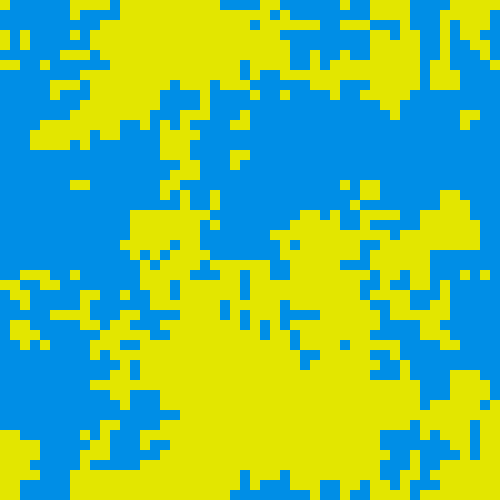
\includegraphics[width=2.2cm]{snapshot2}};
    %%\draw (-2.5,4.2) rectangle (-0.5,2.2);
    %\draw (-1.5,2.15) -- (-4.55,-0.50);
    \node at (-1.25,2.05) {\fbox{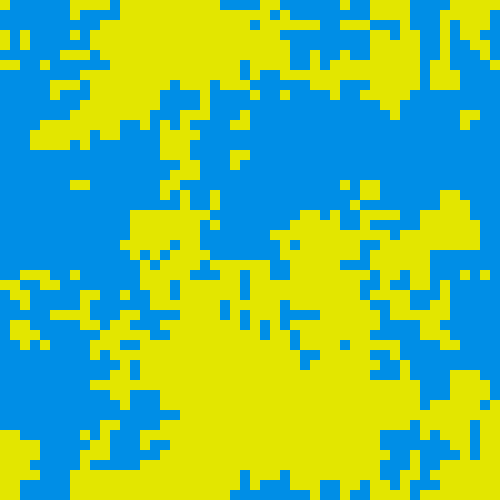
\includegraphics[width=2.2cm]{snapshot2}}};
    %\draw (-2.5,4.2) rectangle (-0.5,2.2);
    \draw (-2.35,2.10) -- (-4.45,-0.40);
    \node at (-4.7,-7.3) {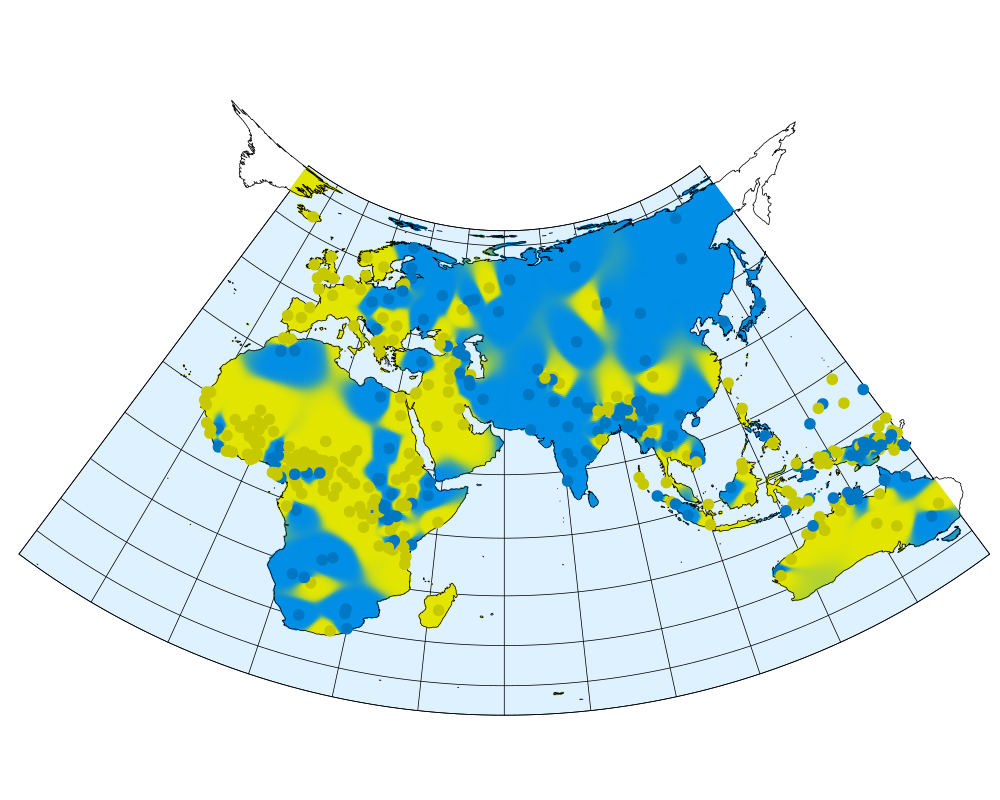
\includegraphics[scale=0.23]{interp_1}};
    \node at (4.5,-7.3) {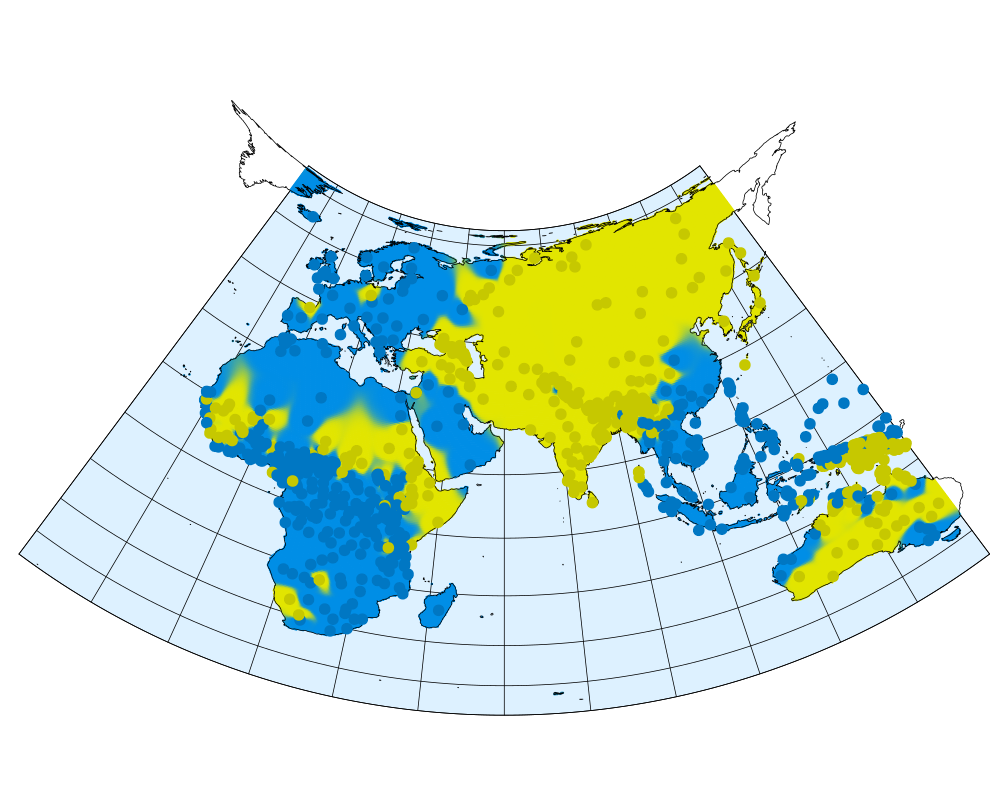
\includegraphics[scale=0.23]{interp_2}};
    \node at (-1.4,3.35) [above] {\textbf{a}};
    \node at (7.8,3.35) [above] {\textbf{b}};
    \node at (-1.4,-5.5) [above] {\textbf{c}};
    \node at (7.8,-5.5) [above] {\textbf{d}};
  \end{tikzpicture}

\end{document}
